\documentclass[]{article}
\usepackage{graphicx}
\usepackage{amsmath}

%opening

\begin{document}

\section{7. Segmentation and Generative Networks}
	\subsection{Segmentation}
		\begin{itemize}
			\item Semantic segmentation: Pixel-level demarcation. No detection
			\item Classification and Localisation: Produce a bounding box around an object and classify it
			\item Object detection: Multiple object classification with bounding boxes
			\item Instance segmentation: Multiple object classification with pixel-level demarcation.
		\end{itemize}
		For the time being we restrict ourselves to talking about semantic segmentation.
		The goal of segmentation is to segment an image into coherent objects. At a high level, we can attempt to group tokens from the 'bottom up' by finding similar neighbour tokens, or the 'top down' by grouping tokens that likely belong to the same object.
	
		\subsubsection{Clustering}
			Clustering can be used to segment images. At a simple level we could simply cluster based on intensity / colour distributions. Other options could be intensity+position, texture (via a filter bank). 
			
			\begin{itemize}
				\item K-means clustering: It's simple and fast to compute, however setting k can be tricky, it is sensitive to outliers and initialisation, and detects spherical clusters (using l2 norm)
				\item Mean-shift clustering: focuses on the mean density, iteratively converges to a region of highest density. This process is more robust to outliers, and has only one parameter, and does not assume shape of clusters. However choosing a window size is tricky, and it does not scale well with dimensions of feature space (curse of dimensionality).
				
				\begin{enumerate}
					\item Define search window radius
					\item For each search window compute the centre of mass
					\item For each search window compute the mean shift vector: $msv_new = C.O.M. - msv_old$ 
					\item Search windows will converge to 'basins' and we merge windows that end up close to each other.
				\end{enumerate}
			\newpage
			\begin{figure}[h!]
				\begin{center}
					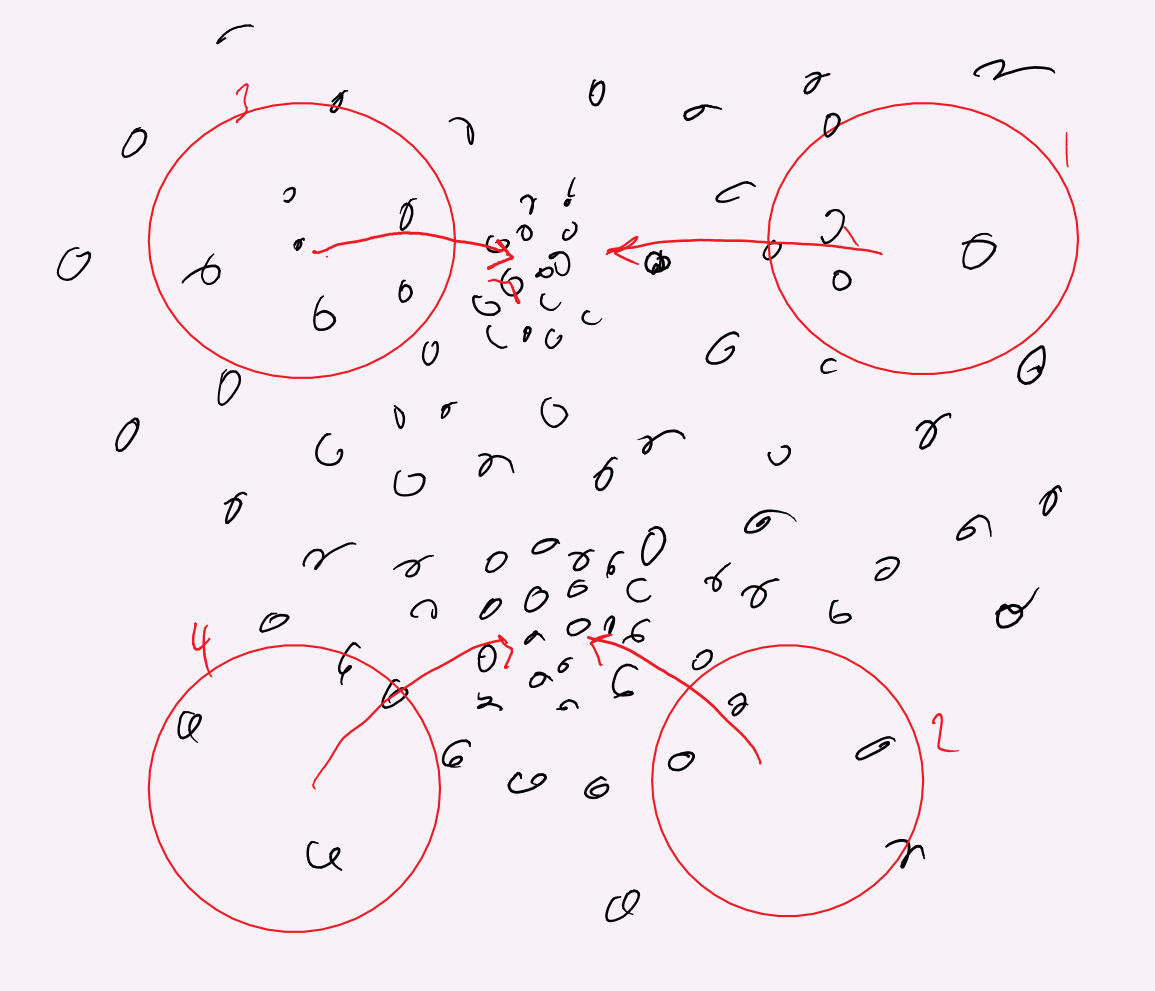
\includegraphics[width=0.5\linewidth]{./images/meanshift.PNG}
					\label{fig:ms}
				\end{center}
			\end{figure}
			
			\begin{center}
				Figure \ref{fig:ms}: Mean shift convergence
			\end{center}
			\end{itemize}
	
	\subsection{End to end: Deep learning approaches}
	
		The task is to output an image mask (with pixel level segmentation). Training requires labelled data set (i.e. gold standard image masks). Two main architectures are described below.
		
		\subsubsection{Fully Connected Network: FCN}
		
			A 'standard' classifier first uses CNN's to extract features, then dense layers to classify. This architecture is similar, except the output of the dense layers now gets upsized to an output layer of the same dimensions as the input image. Skip connections between input and output are added to help with the upsampling.
			
			\begin{figure}[h!]
				\begin{center}
					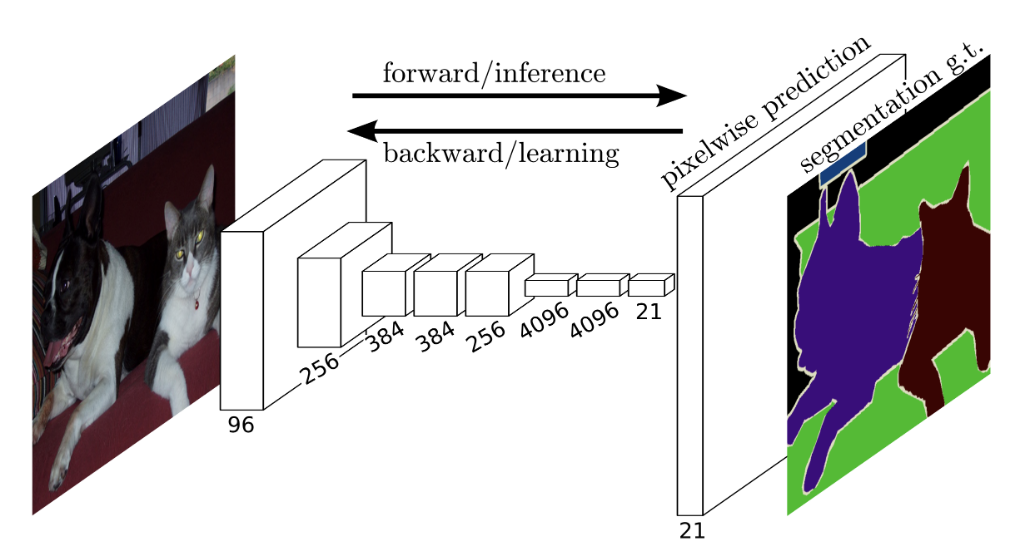
\includegraphics[width=0.5\linewidth]{./images/fcn.png}
					\label{fig:fcn}
				\end{center}
			\end{figure}
			
			\begin{center}
				Figure \ref{fig:fcn}: FCN architecture in a nutshell
			\end{center}
		\newpage
		\subsubsection{U-Net Architecture}
		
			This is similar to an auto-encoder, a symmetry of the network as the input is downsized and then upsized in the same manner. 'Skip connections' are provided between each down/up stage.
			
		\begin{figure}[h!]
			\begin{center}
				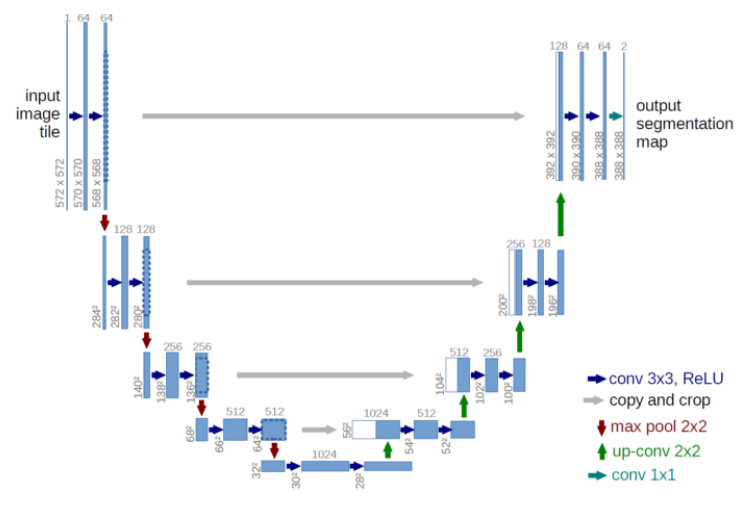
\includegraphics[width=0.5\linewidth]{./images/unet.png}
				\label{fig:unet}
			\end{center}
		\end{figure}
		
		\begin{center}
			Figure \ref{fig:unet}: FCN architecture in a nutshell
		\end{center}
			
\section{Generative Adversarial Networks}

Made up of two networks: a generator and a discriminator.

The generator's task is to produce images from random noise inputs and fool the discriminator. The discriminators task is to catch out the generator.\\

Can be used for super-resolution tasks (SRGAN)\\

The objective function follows minimax principles:\\
\\
$min_g max_d \big( E_{x~p_{data}} [log(D_\theta d (x))] + 	E_{z~p(z)}[ log(1-D_\theta d (G_\theta g (z)))] \big)$\\
\\
\textnormal{Training a GAN is tough:}
\begin{itemize}
	\item The discriminator has an easier job and gets better quick, leading to vanishing gradient
	\item Mode collapse: Too little diversity in the samples generated. If the generator is stuck producing crap; it will continue to produce crap.
	\item lack of convergence
	\item The Loss metric needs to be chosen to correspond to image quality (typical Frechet distance)\\
\end{itemize}
\newpage
\textnormal{Tips for training:}

\begin{itemize}
	\item Batchnorm and ReLU
	\item Try different loss functions
	\item Add noise to the inputs / labels
	\item include similarity to loss function to avoid mode collapse
	\item Use labels when possible (CGAN)
\end{itemize}
	






\end{document}